\chapter{\ac{RF}}
\section{Ingénierie des caractéristiques}

Les principales opérations utilisées pour la génération de caractéristiques à partir des mesures sont les quartiles dont la médiane, le gradient, la séparation en plusieurs parties (\textit{splits}), les traversées de l'étendue de valeurs (\textit{crossings}) et la transformée de Fourier (FFT).

\subsection{Visualisation des mesures}

\begin{figure}['h!']
    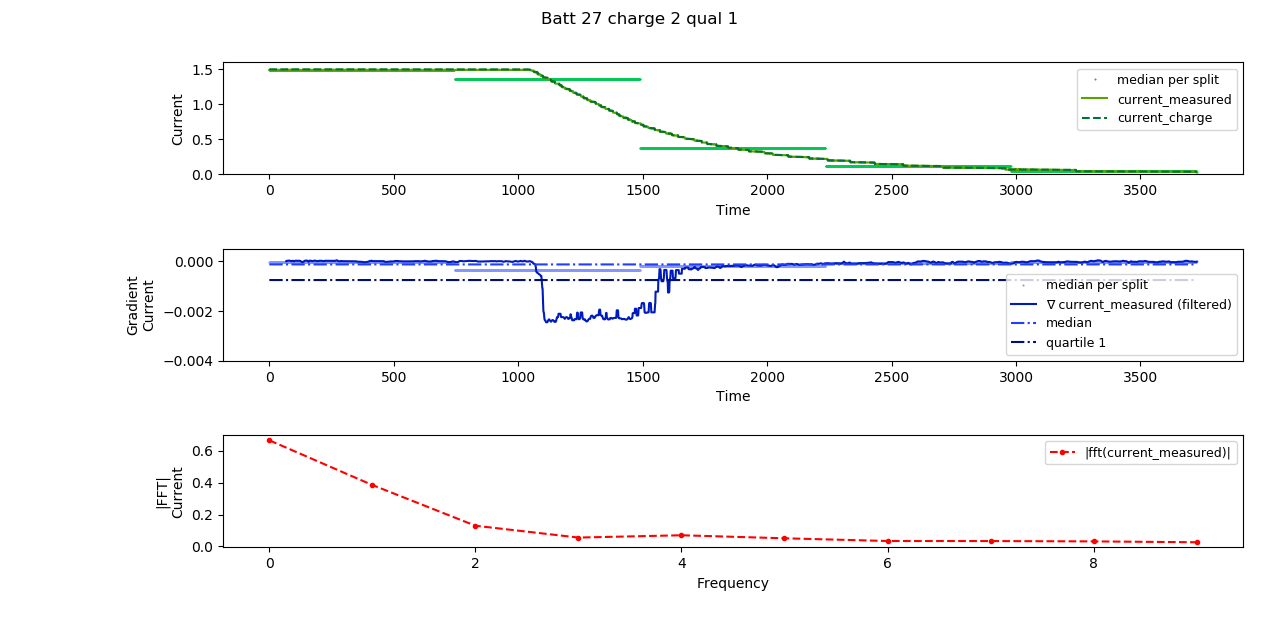
\includegraphics[scale=0.47]{images/rf/batt27_charge2_qual1.png}
    \caption{Qualité 1 -- courant, gradient et FFT}
    \label{fig:RFquality1}
\end{figure}

\begin{figure}['h!']
    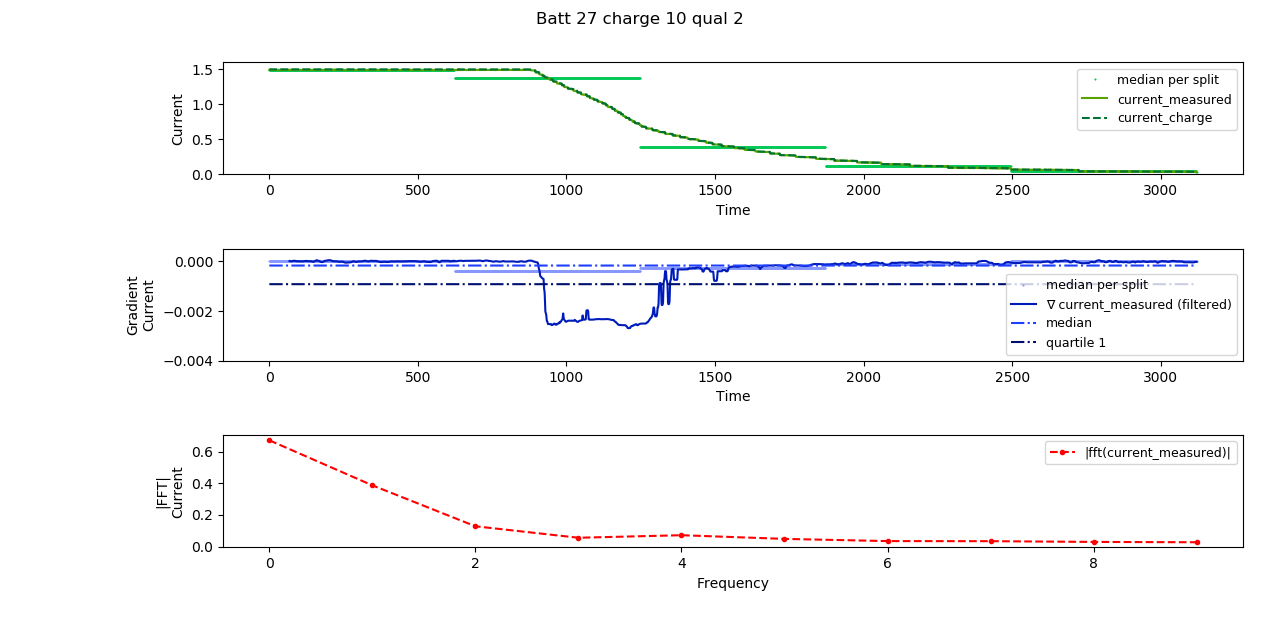
\includegraphics[scale=0.47]{images/rf/batt27_charge10_qual2.png}
    \caption{Qualité 2 -- courant, gradient et FFT}
    \label{fig:RFquality2}
\end{figure}

\begin{figure}['h!']
    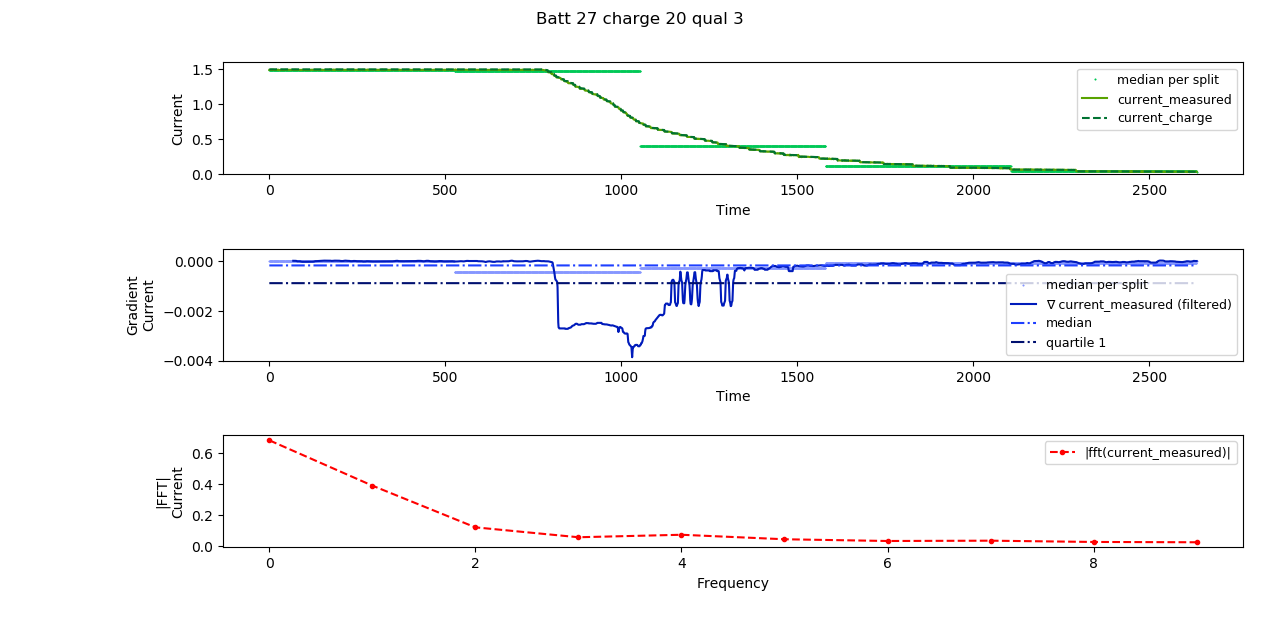
\includegraphics[scale=0.47]{images/rf/batt27_charge20_qual3.png}
    \caption{Qualité 3 -- courant, gradient et FFT}
    \label{fig:RFquality}
\end{figure}

\clearpage

\subsection{Choix des caractéristiques}

De manière générale, les 1er, 3e et 2e quartiles (médiane) ont été utilisés comme un moyen facile de remplacer le minimum, maximum et la moyenne par des notions proches mais robustes face à d'éventuels \textit{outliers}. Cependant le calcul des quartiles est plus coûteux que le calcul du minimum et du maximum.

\subsubsection{Caractéristiques de charge}

\begin{itemize}
    \item Température: différence entre batterie et ambiante.
    \item Tensions, courants: séparation en 5 parts (\textit{splits}).
        \newline {\small Quartiles (1, 3, médiane) et variance pour chaque part: 5 valeurs différentes.}
    \item Tensions, courants: gradient.
        \newline {\small Quartiles (1, 3, médiane) et variance: \textit{5 × la même valeur}}
    \item Tensions, courants: FFT.
        \newline {\small 5 fréquences les plus basses}
    \item Tensions, courants: \textit{crossings}.
        \newline {\small Passages à 25\%, 50\%, 75\% de l’étendue de valeurs (\textit{crossings}).}
\end{itemize}

Il faut noter que dans les caractéristiques de la charge de présentées ici, la médiane (et les quartiles) des gradients du courant et de la tension sont présents 5 fois. Il s'agit d'une erreur lors de la sélection des caractéristiques. Le but était de séparer (\textit{splitter}) ces courbes en 5 puis de calculer les quartiles pour chacune de ces parties. Au lieu de cela on a 5 fois les quartiles (Q1, Q3, médiane) pour chacune de ces courbes. Lorsque je me suis rendu compte de l'erreur, j'ai appliqué la correction afin que le calcul soit fait comme initialement prévu (Q1, Q3 et médiane calculés pour chacune des 5 \textit{splits}), mais pour la charge, cela diminuait le F1-score significativement (de 0.8 à 0.65). Ainsi pour la charge, la correction n'a pas été appliquée et les caractéristiques contiennent 5 fois les quartiles Q1, Q3 et la médiane des gradients du courant et de la tension. Pour la décharge en revanche, la correction a amélioré le F1-score et a donc été conservée.

\subsubsection{Caractéristiques de décharge}
Différences par rapport aux caractéristiques de la charge:
\begin{itemize}
    \item Tensions, courants: gradient puis séparation en 5 parts
        \newline {\small Quartiles (1, 3, médiane) et variance pour chaque part: 5 valeurs différentes.}
    \item Capacité électrique
\end{itemize}

\subsection{Coefficients de Gini}
Un des avantages de l'algorithme Random Forest est qu'il est capable d'indiquer quelles caractéristiques contribuent le plus à l'amélioration du F1-score, sous forme d'un nombre associé à chacune d'elles. Ce sont les coefficients de Gini, qui sont compris entre 0 et 1 et dont la somme vaut 1.

Cette possibilité du Random Forest a été utilisée pour sélectionner les caractéristiques qui maximisent le F1-score: on inclus toutes les caractétistique dont on suppose qu'elles pourraient aider à différencier les bonnes des mauvaises batteries, puis on élimine celles dont les coefficients de Gini sont nuls. Assez souvent le F1-score a augmenté lors de la suppression des caractéristiques dont le coefficient de Gini est nul. Lorsqu'on change les paramètre du RandomForestClassifier, cela vaut la peine de contrôler si les coefficients de Gini des caractéristiques qu'on avait enlevées précédemment sont toujours nuls.

\begin{figure}[h!]
    \centering
    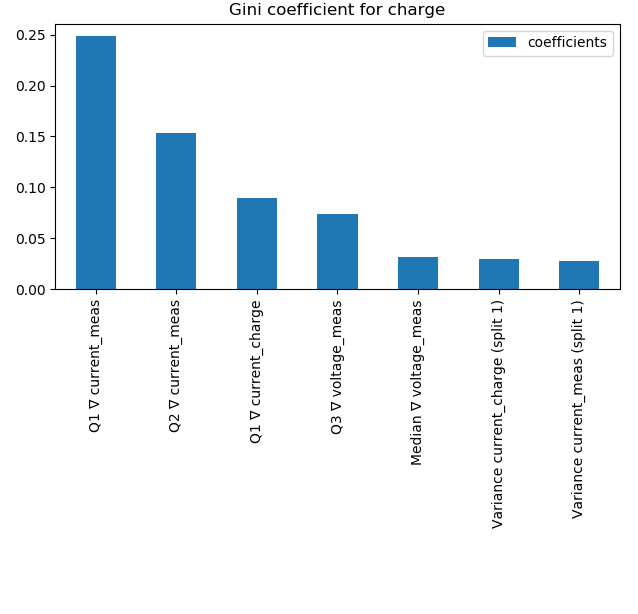
\includegraphics[scale=0.6]{images/rf/gini_charge.png}
    \caption{Coefficients de Gini pour la charge}
    \label{fig:GiniCharge}
    \begin{center}
    Caractéristique la plus influente: variation du courant mesuré.  ($\nabla$ = gradient, Q = quartiles)
    \end{center}
\end{figure}

\begin{figure}[h!]
    \centering
    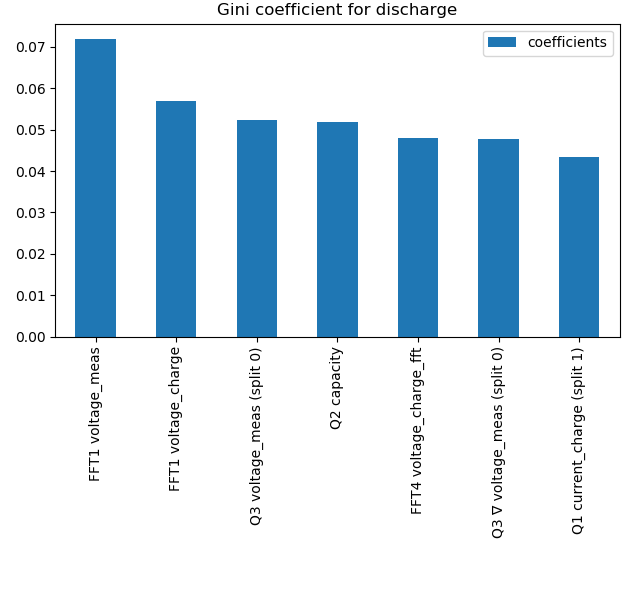
\includegraphics[scale=0.6]{images/rf/gini_discharge.png}
    \caption{Coefficients de Gini pour la décharge}
    \label{fig:GiniDisharge}
    \begin{center}
    Caractéristiques les plus influentes: "fréquences" de la tension, capacité électrique. ($\nabla$ = gradient, Q = quartiles)
    \end{center}
\end{figure}

\clearpage

\section{Procédé}

\begin{figure}[h!]
    \centering
    \makebox[\textwidth]{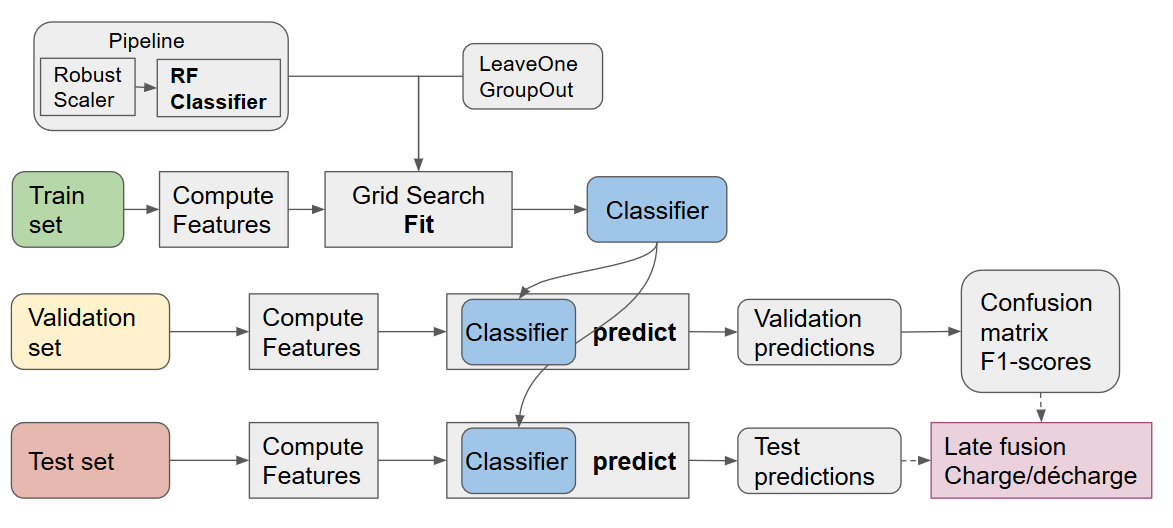
\includegraphics[width=\textwidth]{images/rf/rf_process.png}}
    \caption{Procédé appliqué pour la charge et la décharge respectivement}
    \label{fig:RFProcess}
\end{figure}

Les modèles pour la charge et respectivement la décharge sont construits séparément selon le schéma de la figure \ref{fig:RFProcess}.

Les caractéristiques sont calculées à partir des mesures, puis elles sont normalisées à l'aide d'un RobustScaler.

Le modèle est construit avec une validation croisée \textit{leave one group out} sur les charges (respectivement les décharges) du set d'\textif{entraînement}. Pour effectuer ce \textit{leave one group out}, la normalisation des caractéristiques est intégrée dans un pipeline juste avant le RandomForestClassifier. Ceci est important car les groupes qui sont tour-à-tour laissés de côté dans la validation croisée ne doivent pas influencer les autres groupes.

\begin{minted}{python}
def perform_pipeline_gridsearch(X_train, y_train, n_iter: int, groups) -> RandomizedSearchCV:
    random_grid = build_rf_hyperparams(param_prefix="rf__")
    logo = LeaveOneGroupOut()
    pipeline = Pipeline([
        ("scaler", RobustScaler()),
        ("rf", RandomForestClassifier())
    ])
    clf = GridSearchCV(estimator=pipeline,
                       param_grid=random_grid,
                       cv=logo,
                       iid=False,
                       scoring="f1_macro",
                       return_train_score=False)
    clf.fit(X=X_train, y=y_train, groups=groups)
    return clf
\end{minted}

Un \textit{grid search} est utilisé pour déterminer les paramètres du RandomForestClassifier qui maximisent le F1-score. Une fois le modèle obtenu (\textit{fitté}), on utilise le set de \textif{validation} pour calculer la matrice de confusion ainsi que les F1-scores pour chaque classe.

\clearpage
\section{Résultats}
\subsection{Matrices de confusion}

Les matrices de confusion et les F1-scores ont été calculés avec le set de validation à l'aide des fonctions correspondantes du package \mintinline{python}{sklearn.metrics}.

\subsubsection{Charge}

\begin{figure}['h!']
    \centering
    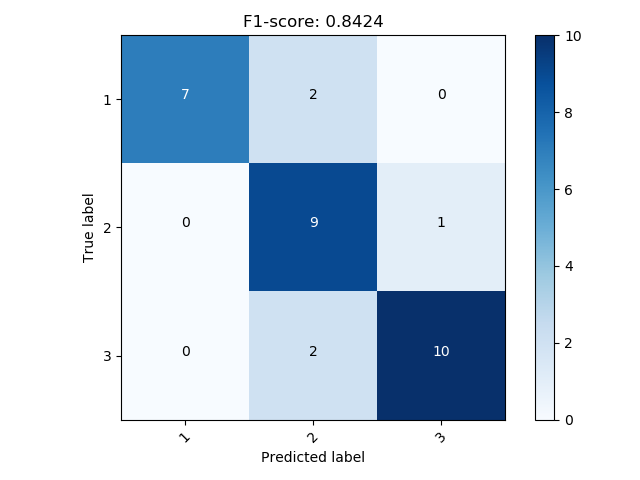
\includegraphics[scale=0.65]{images/rf/cm_charge.png}
    \caption{Matrice de confusion pour la charge}
    \label{fig:RFCMcharge}
    \begin{center}
        F1-score: $0.8424$ (classe 1: $0.88$, classe 2: $0.78$, classe 3: $0.87$).
        \begin{verbatim}
            n_estimators: 10 (arbres), max_depth: 10,
            max_features: sqrt(nb features)}
        \end{verbatim}
    \end{center}
\end{figure}

Le nombre d'arbres a été testé entre 5 et 4000, mais les meilleurs résultats ont toujours été pour un nombre d'arbre relativement faible (entre 10 et 50).

\subsubsection{Décharge}

\begin{figure}['h!']
    \centering
    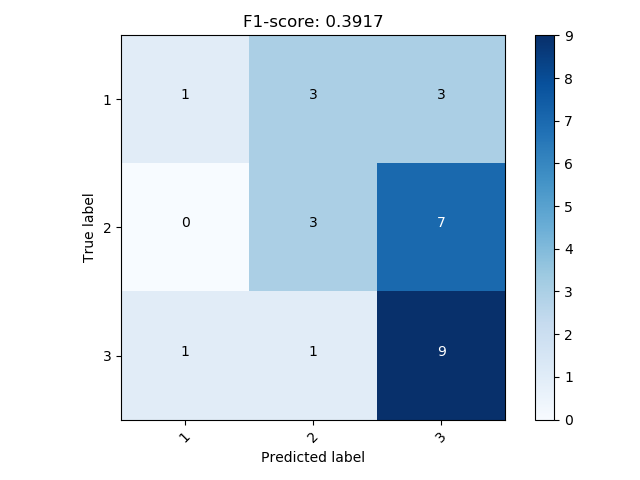
\includegraphics[scale=0.65]{images/rf/cm_discharge.png}
    \caption{Matrice de confusion pour la décharge}
    \label{fig:RFCMdischarge}
    \begin{center}
        F1-score: $0.3916$ (classe 1: $0.22$, classe 2: $0.35$, classe 3: $0.6$).
        \begin{verbatim}
            n_estimators: 5 (arbres), max_depth: 20,
            max_features: log2(nb features)
        \end{verbatim}
    \end{center}
\end{figure}


Tout comme pour la charge, le nombre d'arbres a été testé entre 5 et 4000, mais les meilleurs résultats ont toujours été pour un nombre d'arbre relativement faible (entre 10 et 50).

\section{Fusion des prédiction de charge et décharge}
La principe de \emph{late fusion} a été utilisé pour construire un modèle qui prend en compte les prédictions de charge et de décharge. Ce choix est d'ordre pratique: la prise en compte des données de décharge étant optionnelle dans le cadre du projet, un modèle de prédiction complet a d'abord été construit pour la charge puis a été adapté pour la décharge.

\begin{enumerate}
    \item Calcul du modèle de la charge et des F1-scores de chaque classe (qualité).
    \item Prédiction de la classe pour chaque charge (31 prédictions).
    \item Calcul du modèle de la décharge et des F1-scores de chaque classe (qualité).
    \item Prédiction de la classe pour chaque décharge (28 prédictions).
\end{enumerate}

Pour fusionner les prédiction de charge et décharge, on s'aide de leur ID (\mintinline{python}{charge_nb} et \mintinline{python}{discharge_nb}). En effet, chaque décharge a un ID correspondant à une charge.

Pour chaque prédiction de charge et de décharge (classe 1, 2, 3), on associe le F1-score du modèle pour cette classe. Ensuite, pour chaque charge, on regarde s'il existe une décharge qui a le même ID. Si c'est le cas, on sélectionne la prédiction dont le modèle a le meilleur F1-score. Si une charge n'a aucune décharge qui lui est associée, on garde la prédiction de la charge.

\section{Amélioration}

\begin{itemize}
    \item Affiner le choix des caractéristiques: \newline \textit{grid search} sur les caractéristiques.
    \item Utiliser le pic de la température: d'autres groupes l'ont utilisé et cela s'est révélé efficace.
    \item Inclure le set de validation dans la cross-validation.
    \item Essayer une \textit{early fusion} de la charge et décharge.
\end{itemize}


\section{Conclusion random forest}

Le F1-score obtenu avec les mesures de charge ($0.84$) est meilleur que le F1-score obtenu avec les données de décharge ($0.39$), ce qui est plutôt surprenant. La mise en oeuvre des propositions de la liste d'améliorations devrait permettre d'améliorer le score pour la décharge. De manière général j'ai apprécié travailler sur ce projet car cela m'a permis de me familiariser avec la pratique du machine learning, même si le temps d'investissement est très important.